\section{Anhang}

\subsection{Tabelle Pilzarten} \label{table:shrooms}

\begin{center}
	\begin{tabular}{l | l | l}
		Pilzart & Wissenschaftlicher Name & Essbarkeit\\
		\hline
		Echter Pfifferling/Eierschwamm & Cantharellus cibarius & essbar\\
		Fichten-Reizker & Lactarius deterrimus & essbar\\
		Fichten-Steinpilz & Boletus edulis & essbar\\
		Flaschen-Stäubling & Lycoperdon perlatum & essbar\\
		Fliegenpilz & Amanita muscaria & giftig\\
		Frauen-Täubling & Russula cyanoxantha & essbar\\
		Gemeines Stockschwämmchen & Kuehneromyces mutabilis & essbar\\
		Grüner Knollenblätterpilz & Amanita phalloides & giftig\\
		Herbsttrompete/Totentrompete & Carterellus cornucopioides & essbar\\
		Körnchen-Röhrling & Suillus granulatus & essbar\\
		Maronen-Röhling & Xerocomus badius & essbar\\
		Nebelkappe/Nebelgrauer Trichterling & Clitocybe nebularis & giftig\\
		Perlpilz & Amanita rubescens & essbar\\
		Riesenschirmpilz/Parasolpilz & Macrolepiota procera & essbar\\
		Rötlicher Gallerttrichter & Tremiscus helvelloides & essbar\\
		Rotfuss-Röhrling & Xerocomus chrysenteron & essbar\\
		Schopf-Tintling & Coprinus comatus & essbar\\
		Hallimasch & Armillaria ostoyae & essbar\\
		Spitz-Morchel & Morchella conica & essbar\\
		Wiesen-Egerling/Wiesen-Champignon & Agaricus campestris & essbar\\
	\end{tabular}
\end{center}
\newpage
\subsection{Hochladeformular \& Quiz} \label{img:webpage}

\begin{figure}[h]
	\centering
	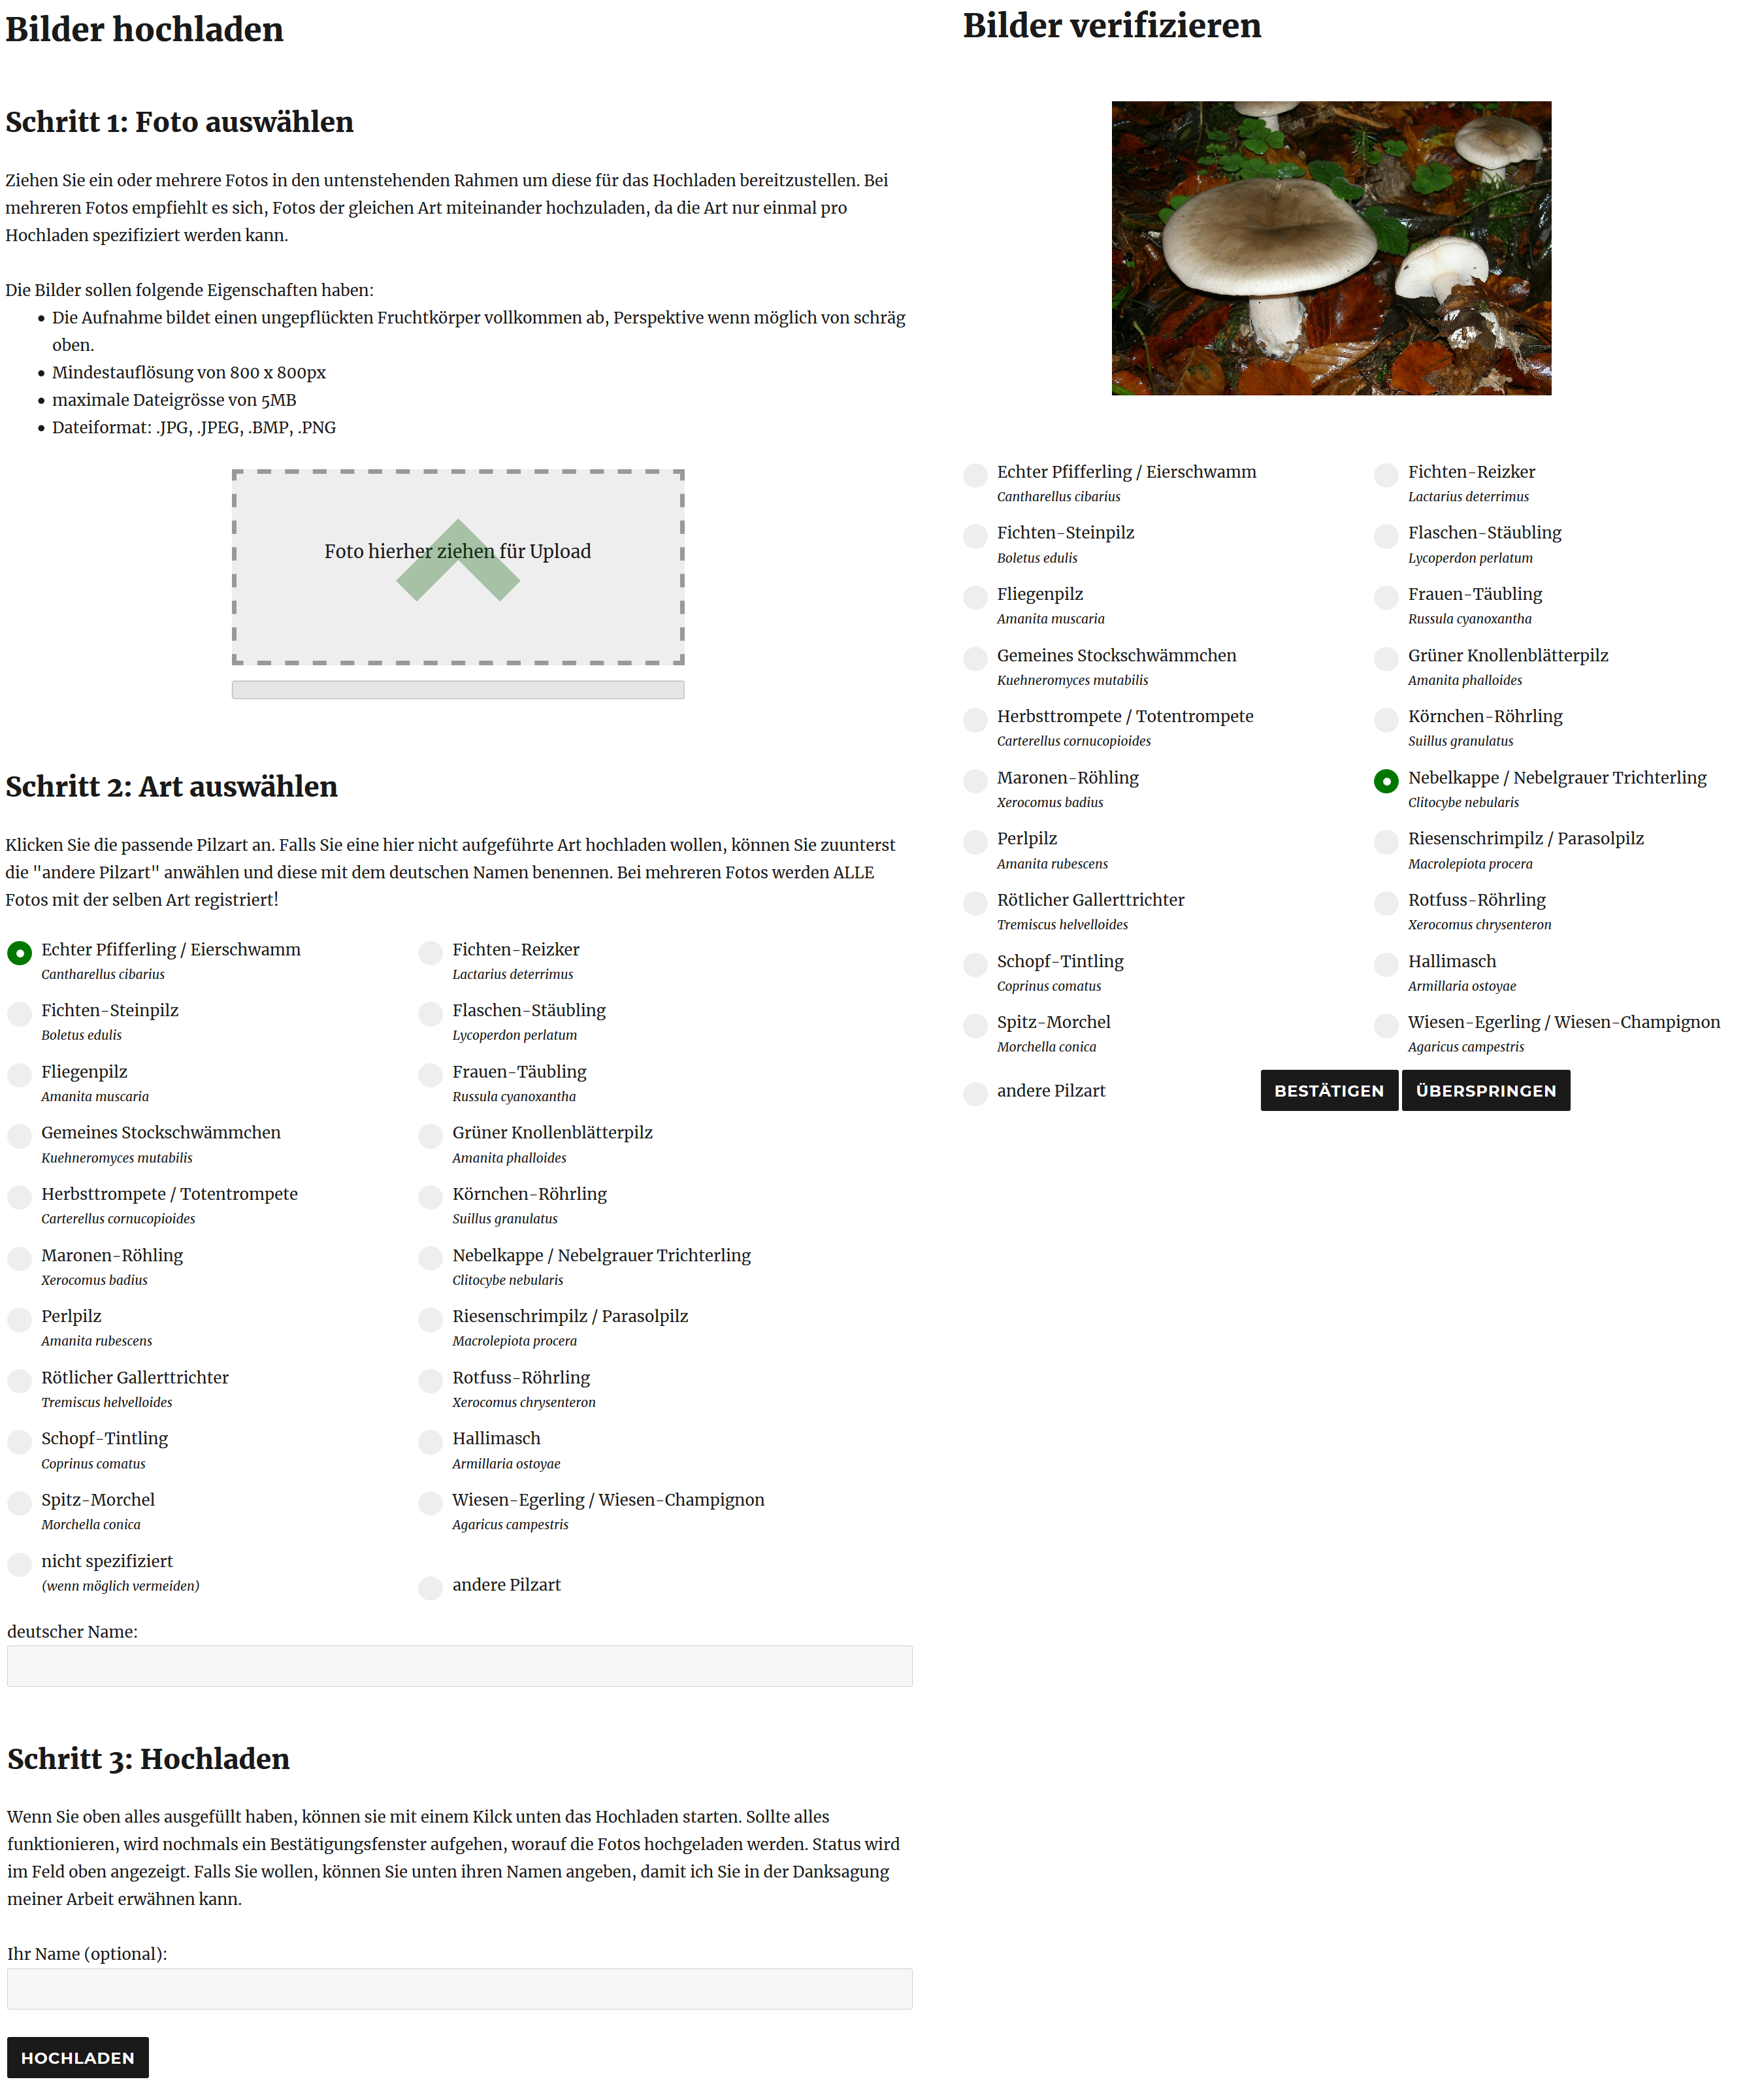
\includegraphics[width=\textwidth]{web_form}
	\caption[\textit{\textit{Hochladeformular \& Quiz}}]{Hochladeformular (links) und Quiz (rechts) von \textit{www.obermeier.ch}}
\end{figure}